\documentclass{standalone}
\usepackage{tikz}
\usetikzlibrary{3d, arrows.meta, positioning}

\begin{document}

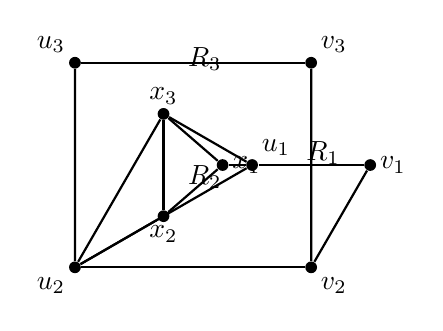
\begin{tikzpicture}[scale=1.5]
  % Vertices
  \node[circle, fill, inner sep=1.5pt] (u1) at (1,0) {};
  \node[circle, fill, inner sep=1.5pt] (u2) at (-0.5,-0.866) {};
  \node[circle, fill, inner sep=1.5pt] (u3) at (-0.5,0.866) {};
  \node[circle, fill, inner sep=1.5pt] (v1) at (2,0) {};
  \node[circle, fill, inner sep=1.5pt] (v2) at (1.5,-0.866) {};
  \node[circle, fill, inner sep=1.5pt] (v3) at (1.5,0.866) {};
  \node[circle, fill, inner sep=1.5pt] (x1) at (0.75,0) {};
  \node[circle, fill, inner sep=1.5pt] (x2) at (0.25,-0.433) {};
  \node[circle, fill, inner sep=1.5pt] (x3) at (0.25,0.433) {};

  % Edges
  \draw[thick] (u1) -- (u2) -- (u3) -- cycle;
  \draw[thick] (v1) -- (v2) -- (v3) -- cycle;
  \draw[thick] (u1) -- (v1);
  \draw[thick] (u2) -- (v2);
  \draw[thick] (u3) -- (v3);
  \draw[thick] (x1) -- (x2);
  \draw[thick] (x2) -- (x3);
  \draw[thick] (x3) -- (x1);
  \draw[thick] (x3) -- (u1);
  \draw[thick] (x3) -- (u2);
  \draw[thick] (x2) -- (u2);
  \draw[thick] (x1) -- (u1);

  % Labels
  \node at (0.6,0.9) {\(R_3\)};
  \node at (0.6,-0.1) {\(R_2\)};
  \node at (1.6,0.1) {\(R_1\)};
  
  \node[below left] at (u2) {\(u_2\)};
  \node[above left] at (u3) {\(u_3\)};
  \node[above right] at (u1) {\(u_1\)};
  \node[below right] at (v2) {\(v_2\)};
  \node[above right] at (v3) {\(v_3\)};
  \node[right] at (v1) {\(v_1\)};
  \node[below] at (x2) {\(x_2\)};
  \node[above] at (x3) {\(x_3\)};
  \node[right] at (x1) {\(x_1\)};
\end{tikzpicture}

\end{document}